%%%%%%%%%%%%%%%%%%%%%%%%%%%%%%%%%%%%%%%%%
% University Assignment Title Page 
% LaTeX Template
% Version 1.0 (27/12/12)
%
% This template has been downloaded from:
% http://www.LaTeXTemplates.com
%
% Original author:
% WikiBooks (http://en.wikibooks.org/wiki/LaTeX/Title_Creation)
%
% License:
% CC BY-NC-SA 3.0 (http://creativecommons.org/licenses/by-nc-sa/3.0/)
% 
% Instructions for using this template:
% This title page is capable of being compiled as is. This is not useful for 
% including it in another document. To do this, you have two options: 
%
% 1) Copy/paste everything between \begin{document} and \end{document} 
% starting at \begin{titlepage} and paste this into another LaTeX file where you 
% want your title page.
% OR
% 2) Remove everything outside the \begin{titlepage} and \end{titlepage} and 
% move this file to the same directory as the LaTeX file you wish to add it to. 
% Then add \input{./title_page_1.tex} to your LaTeX file where you want your
% title page.
%
%%%%%%%%%%%%%%%%%%%%%%%%%%%%%%%%%%%%%%%%%
%\title{Title page with logo}
%----------------------------------------------------------------------------------------
%	PACKAGES AND OTHER DOCUMENT CONFIGURATIONS
%----------------------------------------------------------------------------------------

\documentclass[12pt]{article}
\usepackage[english]{babel}
\usepackage[utf8x]{inputenc}
\usepackage{amsmath}
\usepackage{graphicx}
\usepackage[colorinlistoftodos]{todonotes}

\begin{document}

\begin{titlepage}

\newcommand{\HRule}{\rule{\linewidth}{0.5mm}} % Defines a new command for the horizontal lines, change thickness here

\center % Center everything on the page
 
%----------------------------------------------------------------------------------------
%	HEADING SECTIONS
%----------------------------------------------------------------------------------------

\textsc{\LARGE University of the Witwatersrand}\\[1cm] % Name of your university/college
%\textsc{\Large Major Heading}\\[0.5cm] % Major heading such as course name
%\textsc{\large Minor Heading}\\[0.5cm] % Minor heading such as course title

%----------------------------------------------------------------------------------------
%	TITLE SECTION
%----------------------------------------------------------------------------------------

\HRule \\[0.4cm]
{ \huge \bfseries Reinforcement learning of the Game Pacman}\\[0.4cm] % Title of your document
\HRule \\[1.5cm]
 
%----------------------------------------------------------------------------------------
%	AUTHOR SECTION
%----------------------------------------------------------------------------------------

\begin{minipage}{0.4\textwidth}
\begin{flushleft} \large
\emph{Author:}\\
Tsitsi \textsc{Marote}\\ 856182 % Your name
\end{flushleft}
\end{minipage}
~
\begin{minipage}{0.4\textwidth}
\begin{flushright} \large
\emph{Author:} \\
Meriam \textsc{Elabor} \\1076589 % Supervisor's Name
\end{flushright}
\end{minipage}\\[2cm]

% If you don't want a supervisor, uncomment the two lines below and remove the section above
%\Large \emph{Author:}\\
%John \textsc{Smith}\\[3cm] % Your name

%----------------------------------------------------------------------------------------
%	DATE SECTION
%----------------------------------------------------------------------------------------

%{\large \today}\\[2cm] % Date, change the \today to a set date if you want to be precise

%----------------------------------------------------------------------------------------
%	LOGO SECTION
%----------------------------------------------------------------------------------------


\includegraphics{logo.jpeg}\\[1cm] % Include a department/university logo - this will require the graphicx package
 
%----------------------------------------------------------------------------------------

\vfill % Fill the rest of the page with whitespace

\end{titlepage}


\begin{abstract}
In this research proposal we propose the use of reinforcement learning in training the pacman game. Pacman is an arcade game where the hero tries to eat all the food while avoiding being eaten by monsters. Extra points can be gained for eating the food and the monsters. Reinforcement learning is learning that involves mapping from situations to actions. The learner is not told which action to take, but must learn from the reward system\cite{Introduction}. We wanted an environment that was both intuitive and rich. Pac-Man is intuitive in the sense that it consists of objects moving around on a grid, a setting that can be easily mapped onto the general definitions of search problems and Markov decision processes \cite{teaching}. We are going to consider different ways of representing our states and different reinforcement learning techniques. 
\end{abstract} 

\begin{figure}
\centering
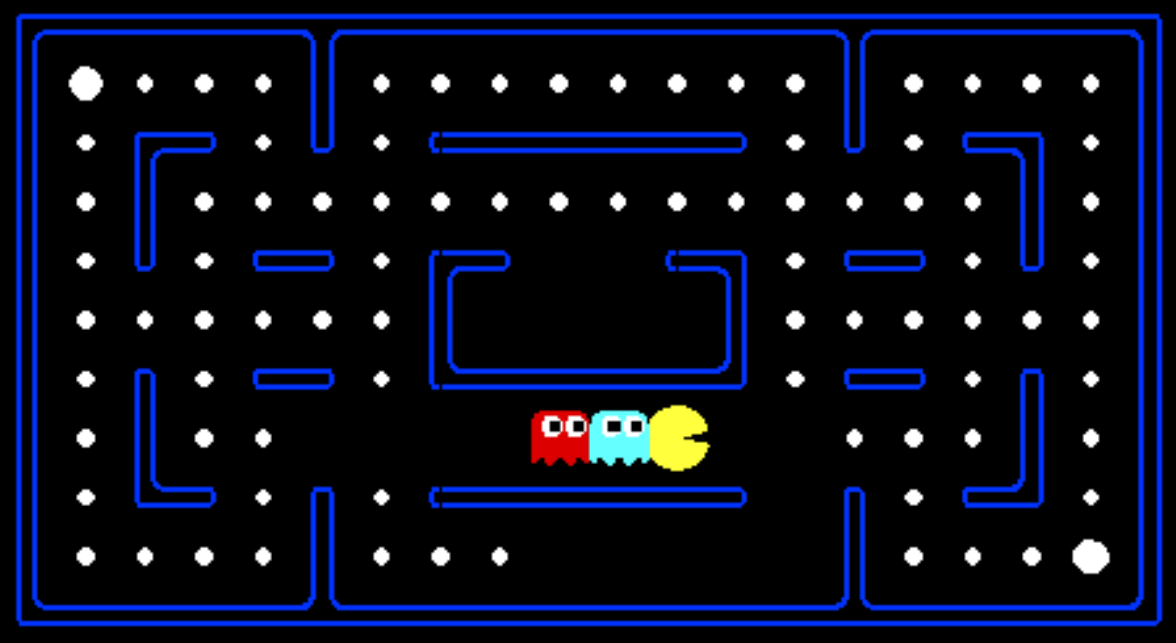
\includegraphics[width=0.3\textwidth]{pacman2.png}
\caption{\label{fig:pacman}Pacman \cite{teaching}.}
\end{figure}


%\section{Application of Reinforcement Learning in Pacman}
%The aim of this research is to implement reinforcement learning to ensure that the pacman makes its own decisions throughout the game. This technique trains the game based on the rewards it gets for moves\cite{Games}. Points will be used to train pacman to know when a move is a good or bad move. Even when multiple moves have been done before getting a reward, pacman still has to be able to tell which moves were good and which ones were bad\cite{Games}. 

\section{Deliverables}
\begin{itemize}
\item Reproduce the pacman game.
\item Create an agent to play the game.
\item Use various techniques to teach the agent.
\item Compare performance. \cite{*}
\end{itemize}

\bibliographystyle{ieeetr}
\bibliography{title_page_1.bib}


\end{document}